% !TeX root = ../main.tex

\chapter{基于区块链技术的访问控制系统BACS}
\label{chap:bacs}

本章首先介绍了基于属性的访问控制模型中的各组成部分以及工作流程,然后介绍了第三方授权认证框架OAuth 2.0的构架和工作流程。在此基础上,本章提出基于区块链的访问控制系统BACS。主要介绍该系统的框架设计和协议流程,以及对安全性进行简要分析。

\section{基于属性的访问控制模型}

基于属性的访问控制ABAC模型主要包含准备阶段和执行阶段,其中准备阶段负责收集访问控制系统中需要的属性集合,以及分析属性之间的关系,构建访问控制策略集合。而执行阶段主要负责验证并回应访问请求,以及对访问控制策略的更新。本文主要研究执行阶段中的访问请求验证步骤,提出基于区块链技术的方案,其他部分采用已有技术。

\begin{figure}[H]
\centering
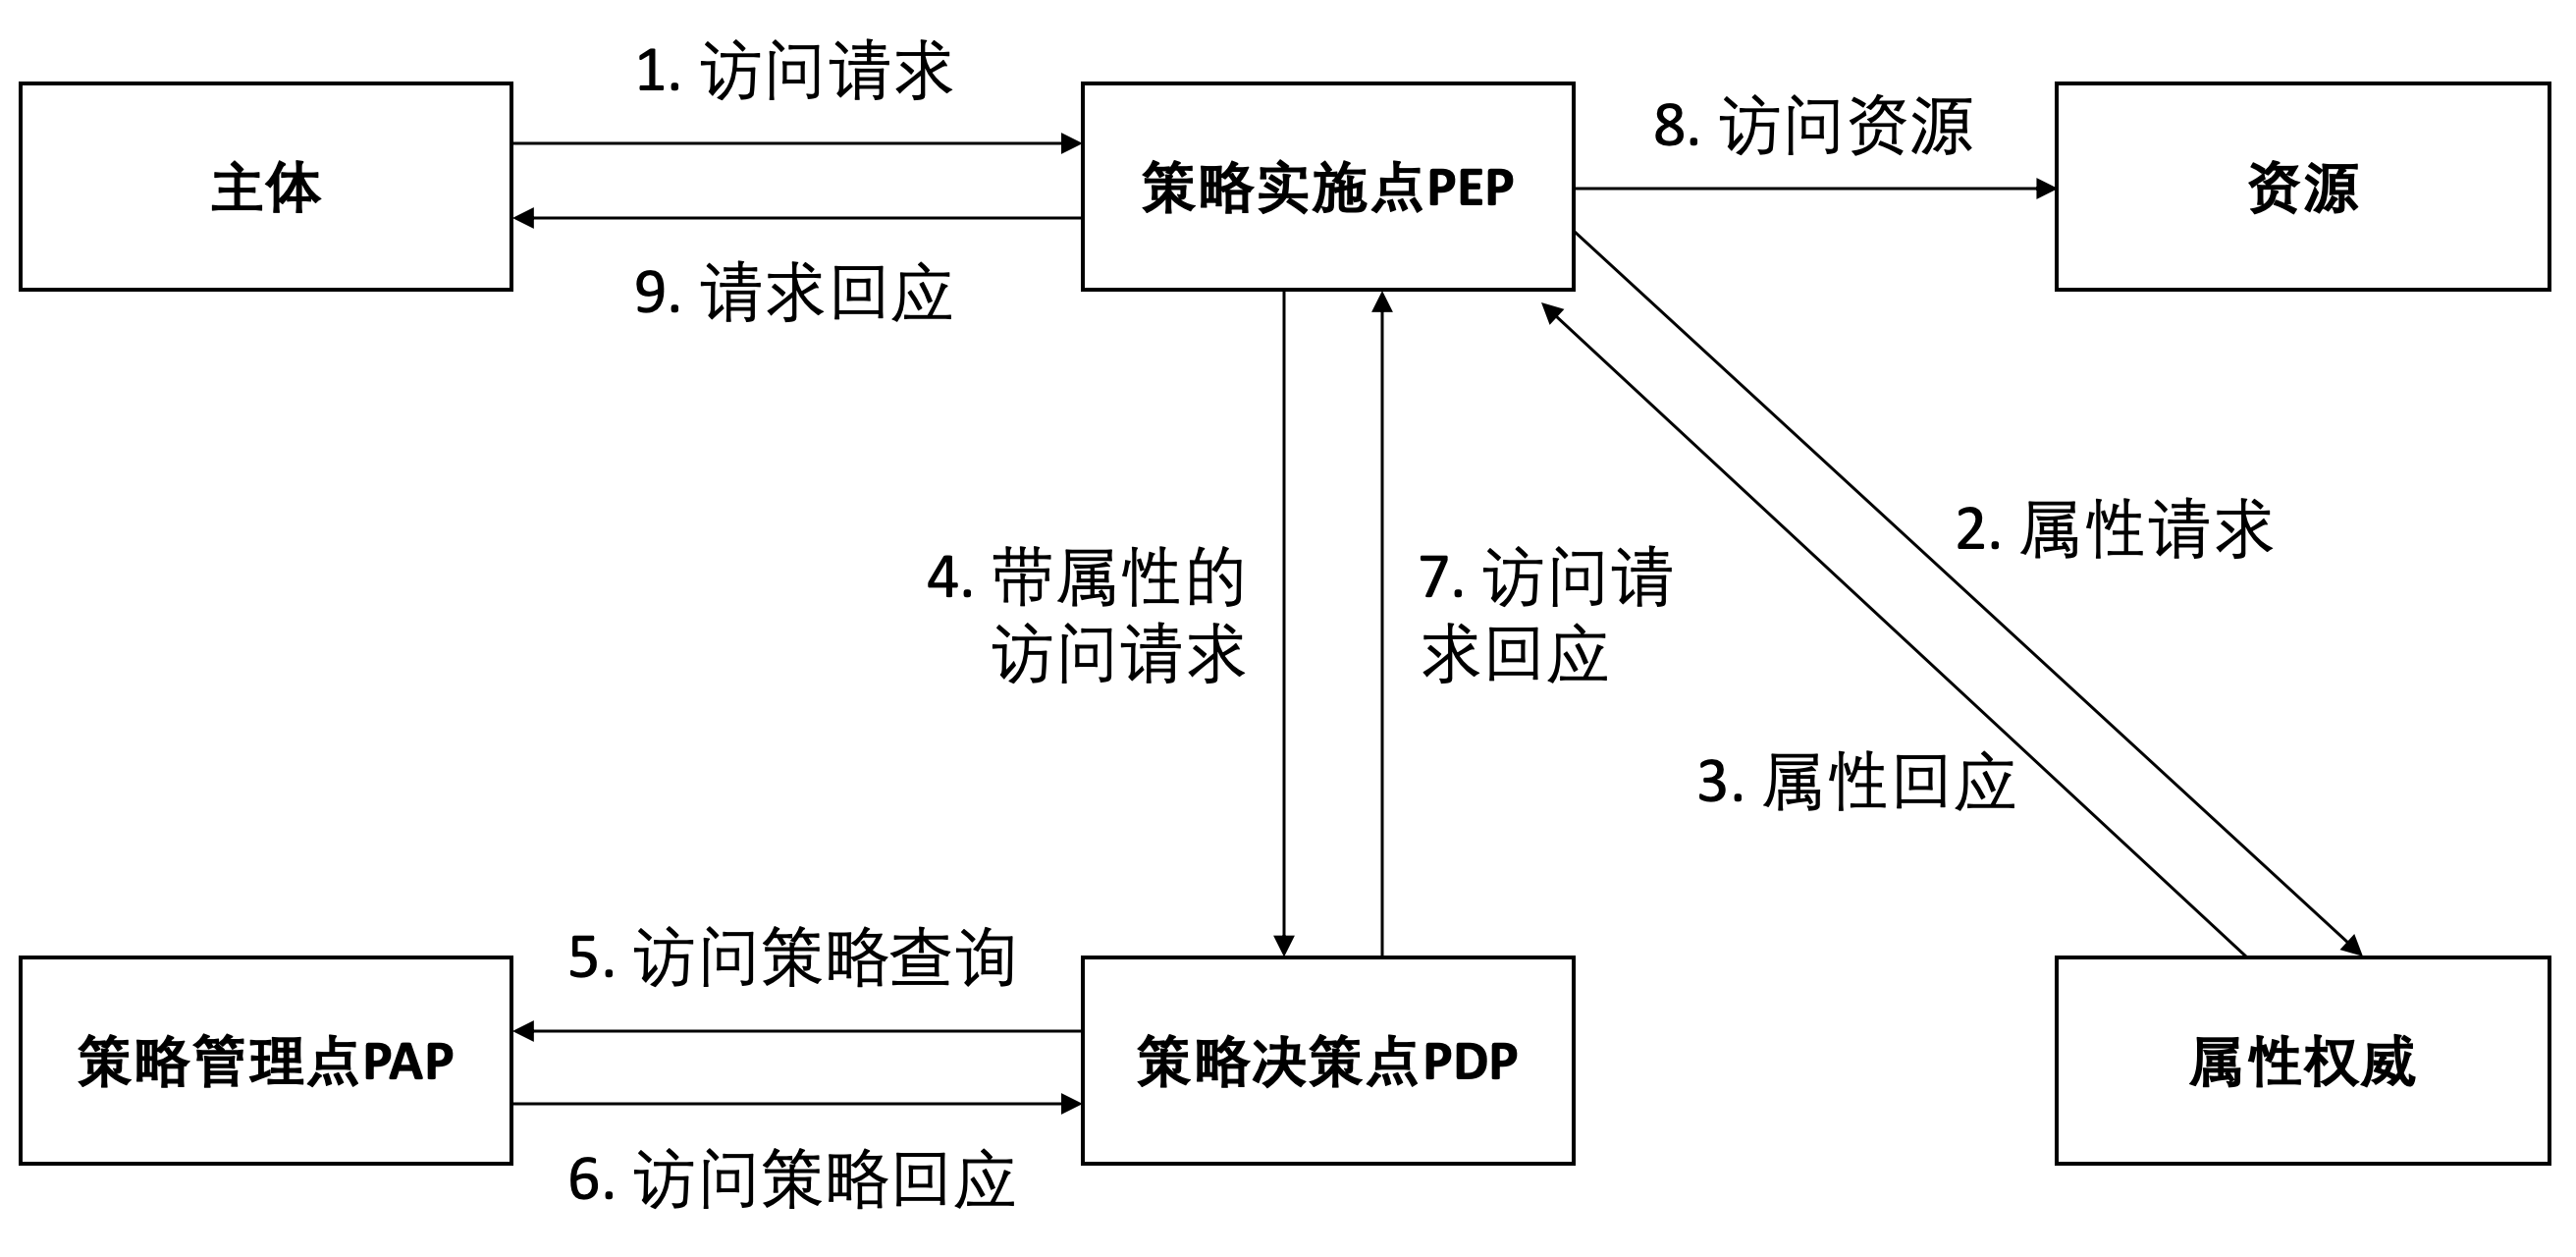
\includegraphics[width=12cm, keepaspectratio]{figures/abac.pdf}
\caption{基于属性的访问控制模型的执行阶段}
\label{fig:abac}
\end{figure}

如图\ref{fig:abac}所示,ABAC模型的访问请求验证主要包含主体,资源,策略实施点(Policy Enforcement Point,PEP),策略决策点( Policy Decision Point,PDP),策略管理点(Policy Administration Point,PAP),属性权威(Attribute Authority)。其中主体表示请求访问资源的用户,策略管理点管理策略列表,包含一系列属性的对应权限逻辑。属性权威返回对于该次请求的主体属性,资源属性,操作属性和环境属性。策略决策点根据请求,从属性权威获取相应的属性值,然后根据策略管理点返回的特定属性策略决策该请求是否通过,策略实施点根据该决策执行相应操作,完成对资源的操作。

\section{第三方授权认证框架}

在互联网时代,网络中各平台分别管理用户的不同数据,为了提升易用性,方便第三方应用访问用户数据,OAuth 2.0框架被各大平台广泛应用。该框架中,主要有客户端,资源所有者,资源服务器和授权服务器四种角色,其中资源所有者将数据存储在资源服务器,给第三方客户端进行授权,客户端通过授权服务器换取凭证,用于访问资源服务器的数据。

\begin{figure}
\centering  
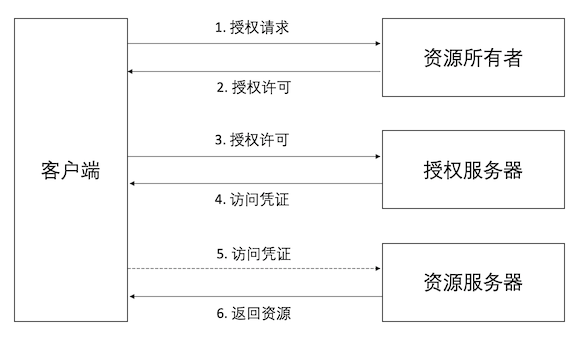
\includegraphics [width=11cm]{figures/oauth.pdf}
\caption{OAuth 2.0框架中授权码模式的正常工作流程}
\label{fig:oauth}
\end{figure}

这里主要介绍OAuth 2.0框架中授权码模式的正常工作流程。如图\ref{fig:oauth}所示,该流程主要有以下3个阶段:

\begin{enumerate}
  \item 客户端向资源所有者发送授权请求,请求获取相应的资源访问权限。资源所有者收到请求后,检查请求的权限,通过验证后返回对应的授权许可给客户端。
  \item 客户端将授权许可发送给授权服务器,授权服务器验证后将对应资源的访问凭证返回给客户端。
  \item 客户端将访问凭证发送给资源服务器,资源服务器验证凭证后执行相应操作,并将结果返回给客户端。
\end{enumerate}

OAuth框架可以支持细粒度、动态和灵活的特权管理,适用于各种访问控制模型,在Google和Facebook等许多公司广泛使用。然而,整个授权认证过程依赖于中心化的授权服务器,存在内部和外部攻击的安全风险。

\section{访问控制系统BACS}

为了解决传统授权服务中存在中心化授权服务器的问题,本文提出基于区块链的访问控制系统BACS,采用联盟链代替中心化的授权服务器,存储管理授权数据记录,增强系统安全性和可信性。本节主要介绍该系统的框架设计,协议流程以及对安全性进行简要分析。

\subsection{第三方授权框架}

\begin{figure}
\centering
\includegraphics[width=14cm]{figures/framework.pdf}
\caption{第三方授权服务框架图}
\label{fig:framework}
\end{figure}

如图\ref{fig:framework}所示,BACS系统包含三类角色,“客户端”作为资源请求者,它请求资源所有者进行授权,并最终请求区块链节点访问资源。“资源所有者”在区块链节点上存储资源,在需要时授予“客户端”访问受保护资源的权限。BACS系统用“区块链节点”组成的联盟网络代替OAuth框架中的中心化认证服务器和资源服务器,每个节点具有平等的地位,由资源服务器和授权服务器组成。其中资源服务器存储用户不同的资源,授权服务器共同参与用户授权数据的存储和管理。

\begin{description}
  \item[\textbf{资源所有者}] 资源所有者存储自己的资源在资源服务器,并在需要时授予客户端访问受保护资源的权限。
  \item[\textbf{客户端}] 客户端指资源请求者,通过向资源所有者发送请求获取授权,并访问资源服务器获取资源。不同于OAuth框架中客户端需要提前注册,任何用户都可以独自创建账户作为客户端。
  \item[\textbf{区块链节点}] 联盟链网络由若干互联的区块链节点组成。每个节点包含授权服务器和资源服务器。其中资源服务器分别存储资源所有者的不同资源,并采用ABAC模型验证操作请求。所有节点的授权服务器共同运行共识协议,管理记录资源所有者对客户端的授权,并维护账户的属性状态。
\end{description}

\subsection{第三方授权服务工作流程}
\label{sec:protocols}
本节介绍BACS系统中授权服务的工作流程。整个协议主要分为5个步骤,分别对应于图\ref{fig:framework}中的工作流程。具体步骤如下:

\begin{enumerate}
  \item 客户端向资源所有者发送$Authorization Request$,其中主要包含客户端的地址和请求授权的属性。
  \item 资源所有者检查$Authorization Request$,如果同意则生成相应的$Authorization Grant$并且发送给任何区块链节点。
  \item 如果接收到的$Authorization Grant$有效,则区块链节点将接受并在网络中传播它。共识过程结束后,授权将被打包到一个新的区块中,并记录到区块链上。
  \item 获得授权后,客户端找到存储需要访问资源的区块链节点,并发送$Operation Request$给该节点的资源服务器。
  \item 资源服务器根据授权服务器提供区块链上账户的主体属性,存储的资源属性以及基于属性的访问控制策略来验证$Operation Request$,根据验证结果回应客户端。
\end{enumerate}

接下来将详细介绍各步骤的细节。首先介绍后续涉及的一些密码学表示,对于消息$m$,我们定义$H(m)$表示$m$的哈希值,并且用$\langle m \rangle_{\sigma_{i}}$ 表示消息 $m$ 以及节点$i$对 $H(m)$ 的签名。可以用于验证该消息的真实来源以及是否在传输中被篡改。

\subsubsection{区块链和属性状态}

该系统中,区块链是用来存储授权记录的基本数据结构,每个区块记录一系列授权信息,每个授权信息包括发送方地址,接收方地址,授权属性,授权有效期以及用于验证的签名等信息。为了在本系统中,我们采用了以太坊项目中的账户状态机制,而非比特币项目中的未花费输出UTXO(Unspent Transaction Output)机制,因为状态设计更适合ABAC模型。我们将账户中的余额等信息修改为属性状态,区块链记录每个账户拥有的所有属性以及nonce值,每个属性包括属性名和有效期。

根据区块链上记录的信息,我们可以计算包含地址、nonce和属于地址的属性状态的每个帐户的状态。状态保存在内存中,可用于验证授权或操作。在区块链上添加新块时,全局状态将根据新块中的授权进行更改。我们可以将全局状态视为区块链的当前结果。对于帐户状态中的$nonce$值,每个帐户都有一个$nonce$值,其值为0。地址D的一次授权记录在区块链上时,地址D的一次授权将增加1。任何与nonce值不匹配的授权都将被拒绝,可以防止重播攻击。

\subsubsection{区块生成算法}

 \begin{algorithm}
 \floatname{algorithm}{Algorithm}{}
 \caption{Block Generation}\label{alg:blockGeneration}
   \begin{algorithmic}[!htbp]
   \renewcommand{\algorithmicrequire}{\textbf{Input:}}
   \renewcommand{\algorithmicensure}{\textbf{Output:}}
   \REQUIRE $AuthorizationPool, AUTH\_LIMIT, PreviousBlock$
   \ENSURE  $Verification$
    \STATE $auths \gets ChooseAuths(AuthorizationPool, AUTH\_LIMIT)$
    \STATE $prevHash \gets H(PreviousBlock)$
    \STATE $timestamps \gets CurrentTime()$
    \STATE $newBlock \gets NewBlock(prevHash, auths, timestamps)$
   \RETURN $newBlock$
   \end{algorithmic}
 \end{algorithm}

联盟网络中的节点会将一段时间内接受到的授权信息打包到一个新区块中,在比特币系统中这个时间间隔是10分钟,而在以太坊中是15秒,动态调整的具体方法在前文章节中有所介绍。而在本系统中,为了保障访问控制系统的延迟可接受,我们设置区块间隔为2秒,区块生成的具体算法在算法\ref{alg:blockGeneration}中介绍。

\subsection{改进的PBFT共识协议}
\label{subsec:adapted-pbft}

在前文第\ref{subsec:traditional-consensus}节中,我们介绍了多种共识协议。我们在访问控制系统中采用了改进的PBFT协议。区块链网络广播中的节点向其他节点发送请求。经过一段时间后,主节点将合法请求打包成块。然后将该块广播到网络中,与其他节点达成共识。

主节点、备份节点和视图更改基本采用PBFT协议的设计。但针对区块链技术需求进行以下改进,PBFT协议中的主节点在接收到来自客户端的请求时开始协商过程。BACS系统中,主节点每2秒启动一次协商,并将最多1000个授权打包到一个新区块中。当备份节点发现主节点似乎发生故障或被攻击时,将发生视图更改,这与PBFT协议中的视图变化相同。除此之外,当一段时间后,系统中的节点也会自动进行视图更改。这可以防止来自恶意主节点的黑名单攻击。在区块链系统中,生成新块的节点可以选择其中包含的事务以及先后顺序,恶意节点可以拒绝打包黑名单中帐户的事务。因此,不断的视图更改可以防止来自恶意主节点的黑名单攻击。改进的PBFT共识协议中设计了各类消息的数据结构,如图\ref{fig:pbft-data}所示。接下来介绍各阶段的具体实现算法。

\begin{figure}
  \centering%
  \subcaptionbox{“预准备消息”数据结构\label{fig:pre-prepare}}
    {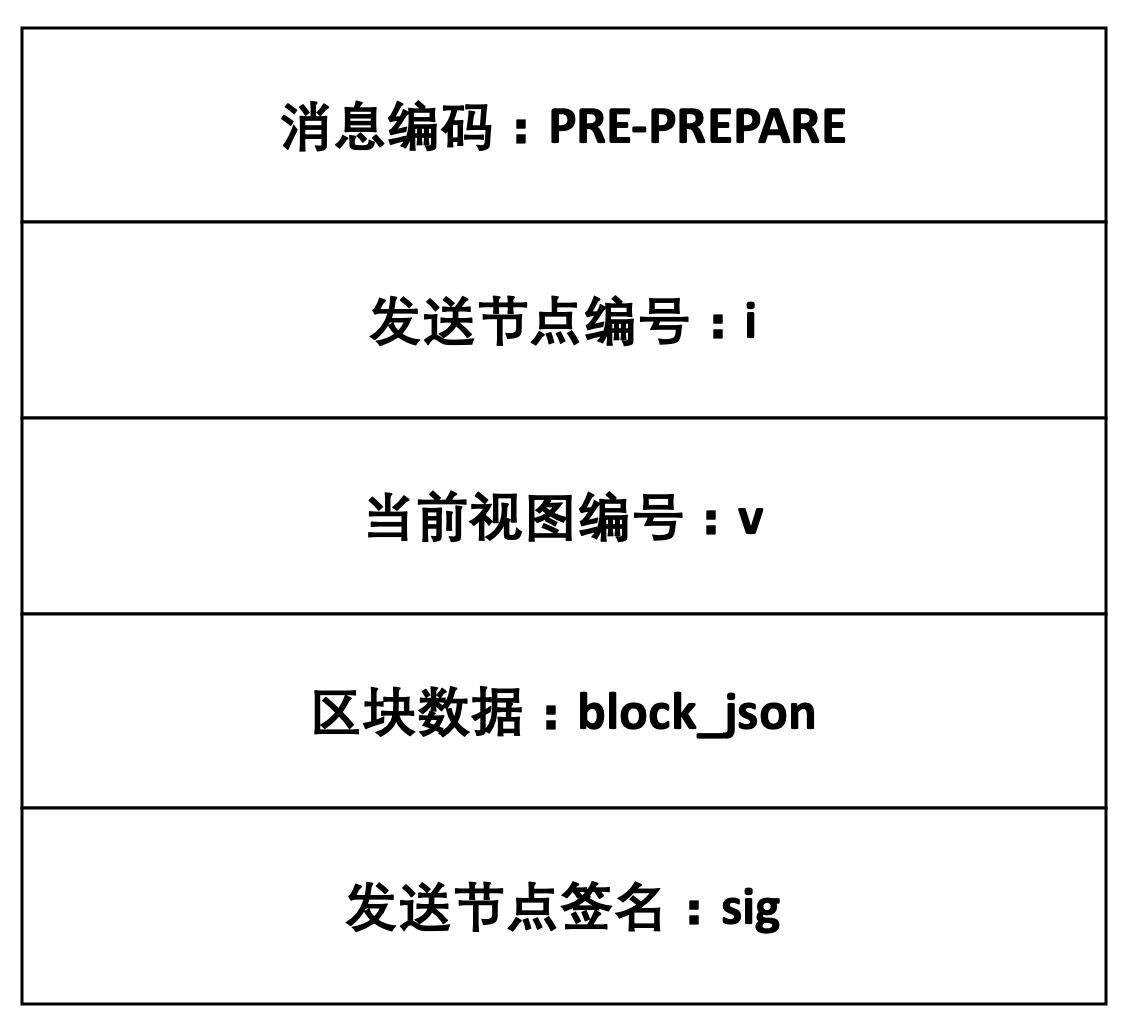
\includegraphics[width=6cm]{figures/pre-prepare.pdf}}%
  \hspace{2em}%
  \subcaptionbox{“准备消息”数据结构\label{fig:prepare}}
      {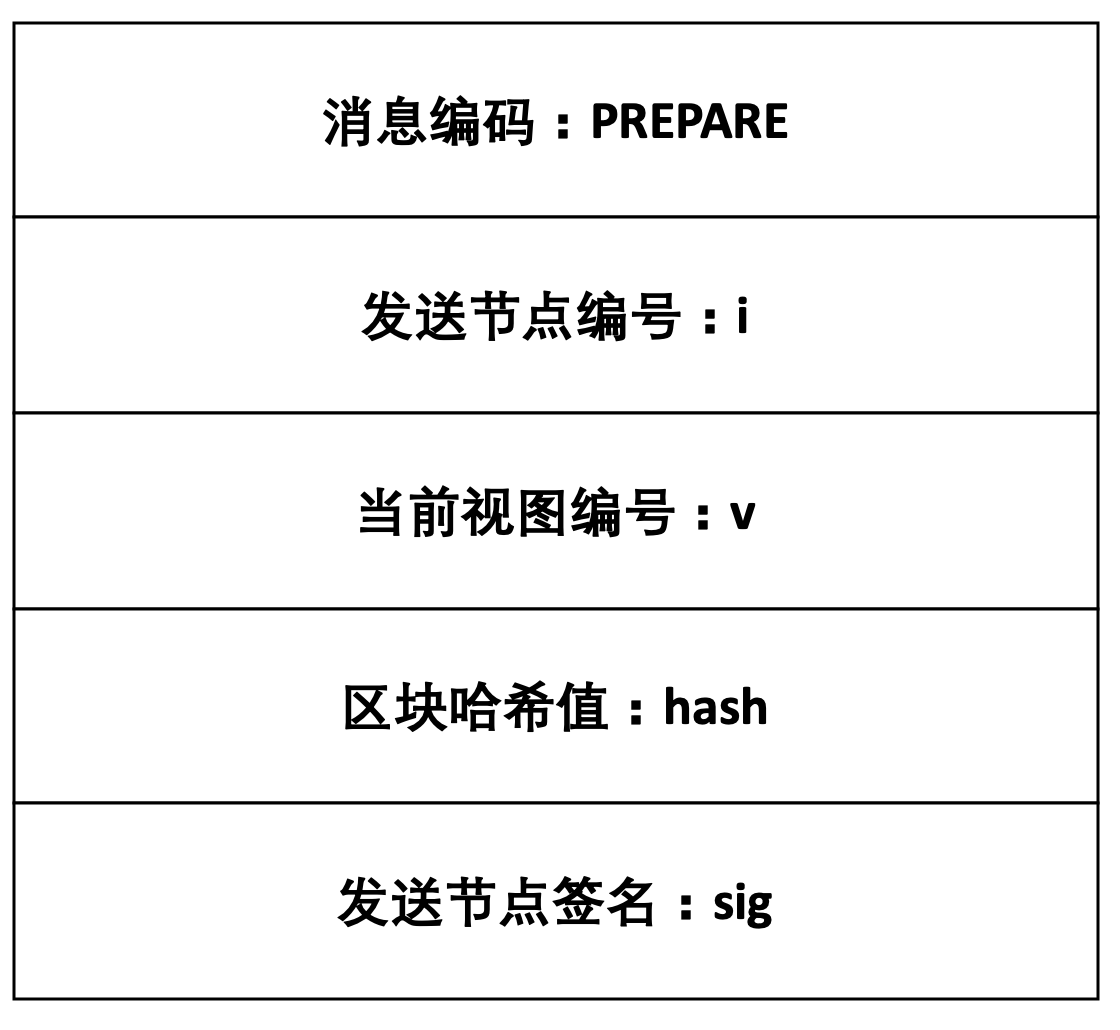
\includegraphics[width=6cm]{figures/prepare.pdf}}

  \subcaptionbox{“承诺消息”数据结构\label{fig:commit}}
      {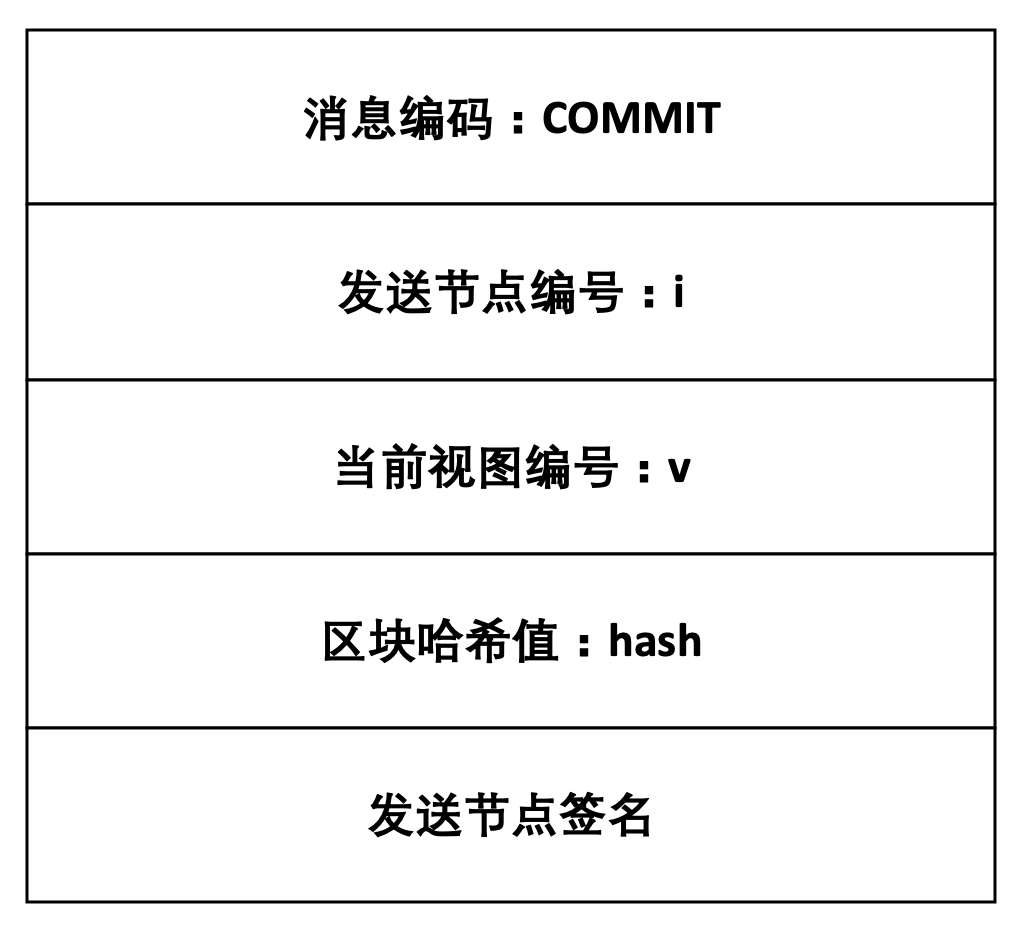
\includegraphics[width=6cm]{figures/commit.pdf}}
  \hspace{2em}%
  \subcaptionbox{“视图更新消息”数据结构\label{fig:viewchange}}
      {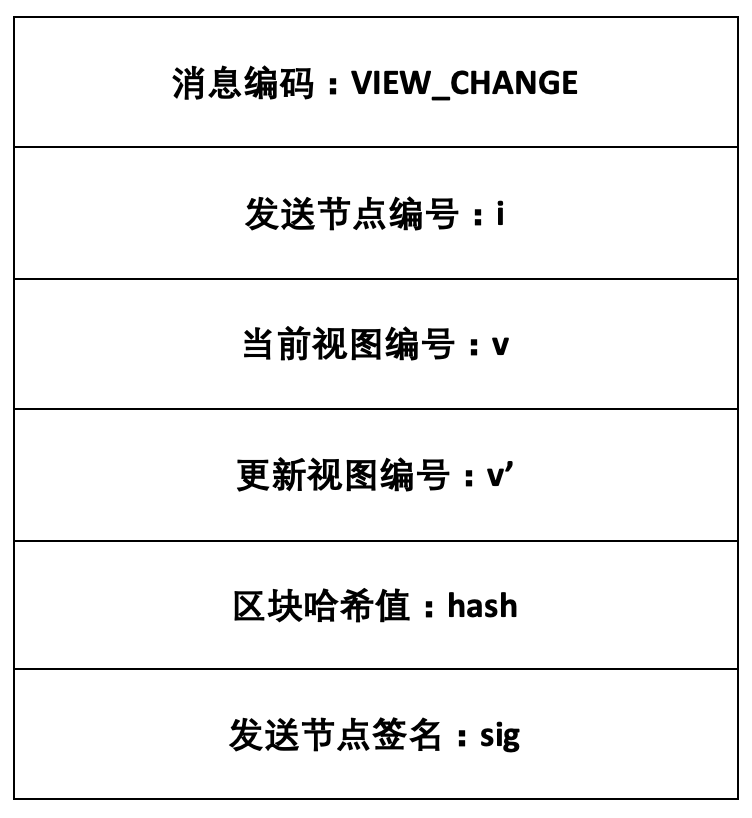
\includegraphics[width=6cm]{figures/viewchange.pdf}}
  \caption{共识协议中各类消息的数据结构}
  \label{fig:pbft-data}
\end{figure}

\subsubsection{预准备阶段}

 \begin{algorithm}
 \floatname{algorithm}{Algorithm}
 \caption{生成预准备信息}\label{alg:preprepareGen}
   \begin{algorithmic}[H]
   \renewcommand{\algorithmicrequire}{\textbf{Input:}}
   \renewcommand{\algorithmicensure}{\textbf{Output:}}
   \REQUIRE $blockchain, authorizationPool, AUTH\_LIMIT,$ $sk, viewID$
   \ENSURE  $pre$-$prepare$
    \STATE $prevBlock \gets blockchain.LastBlock()$
    \STATE $block$ $\gets$ $BlockGenration(prevBlock, AUTH\_LIMIT,$ $authorizationPool)$
    \STATE $pre$-$prepare \gets NewRequest(viewID, block)$
    \STATE $signature \gets sk.Sign(request)$
    \STATE $pre$-$prepare.Signature \gets signature$
   \RETURN $pre$-$prepare$
   \end{algorithmic}
 \end{algorithm}

当一个新区块过程开始,所有节点进入预准备阶段。这一阶段中,主节点从授权池中选择一系列合法的授权,并且打包到一个新区块中。然后,主节点广播预准备信息$\langle PRE$-$PREPARE, v, i, block \rangle_{\sigma_{i}}$ 给所有备份节点,其中 $v$ 表示当前的视图编号,$i$ 表示主节点的节点编号。具体预准备信息$pre$-$prepare$的创建如算法\ref{alg:preprepareGen}所示。

 \begin{algorithm}[H]
 \floatname{algorithm}{Algorithm}
 \caption{验证预准备信息}
   \begin{algorithmic}[H]\label{alg:prepreVerify}
   \renewcommand{\algorithmicrequire}{\textbf{Input:}}
   \renewcommand{\algorithmicensure}{\textbf{Output:}}
   \REQUIRE $pre$-$prepare$, $N$, $ViewID$, $i$, $PkList$
   \ENSURE  $Verification$
    \STATE $viewID$, $nodeID$, $timestamps$, $signature \gets Parse(pre$-$prepare)$
    \IF {$viewID \ne ViewID$}
      \RETURN $false$
    \ENDIF

    \IF {$nodeID \ne ViewID \% N$}
      \RETURN $false$
    \ENDIF

    \STATE $hash \gets H(pre$-$prepare)$
    \IF {$CheckSignature(PkList[i], hash, signature) \ne true$}
      \RETURN $false$
    \ENDIF
   \RETURN $true$
   \end{algorithmic}
 \end{algorithm}

当备份节点接受到主节点发送的预准备信息$pre$-$prepare$后,验证过程如算法\ref{alg:prepreVerify}所示。如果通过验证,备份节点将接受该信息并进入准备阶段。否则,该节点可以认为主节点被恶意控制或者宕机,将会发起视图切换,请求选举出下一个正常节点作为新的主节点。

\subsubsection{准备阶段}

 \begin{algorithm}
 \floatname{algorithm}{Algorithm}
 \caption{生成准备信息}
   \begin{algorithmic}[H]\label{alg:prepareGen}
   \renewcommand{\algorithmicrequire}{\textbf{Input:}}
   \renewcommand{\algorithmicensure}{\textbf{Output:}}
   \REQUIRE $pre$-$prepare, nodeID, sk, NeighborList$
   \ENSURE  $prepare$

    \STATE $blockHash$ $\gets$ $H(pre$-$prepare.Block)$

    \STATE $viewID \gets pre$-$prepare.ViewID$
    \STATE $prepare \gets NewPrepare(viewID, nodeID, blockHash)$
    \STATE $signature \gets sk.Sign(prepare)$
    \STATE $prepare.Signature \gets signature$
   \RETURN $prepare$
   \end{algorithmic}
 \end{algorithm}

如果备份节点 $i$ 接受了预准备信息$pre$-$prepare$,该节点进入准备阶段。节点$i$生成准备信息$\langle PRE$-$PARE, v, i, blockHash\rangle_{\sigma_{i}}$,其中视图编号$v$和预准备信息中的视图编号一致,$i$ 表示该备份节点的节点编号,$blockHash$ 表示预准备信息$pre$-$prepare$中包含区块的哈希值。具体细节在算法\ref{alg:prepareGen}中介绍。然后该备份节点将生成的准备信息 $prepare$广播给其他所有节点,包括主节点在内。一旦某个节点从不同的来源节点(包括自己)接收到$2f+1$个拥有相同$v$和 $blockHash$的准备信息,该节点将会进入承诺阶段。

\subsubsection{承诺阶段}

进入承诺阶段的节点获知网络中大部分正常节点(至少f+1个)已经接受该信息。节点$i$将生成并广播承诺信息$\langle COMMIT, v, i, blockHash \rangle_{\sigma_{i}}$ 给所有节点,表明该节点将接受这一新区块作为共识结果。承诺的生成过程如算法\ref{alg:commitGen}所示。

 \begin{algorithm}
 \floatname{algorithm}{Algorithm}
 \caption{Commit Generation}
   \begin{algorithmic}[H]\label{alg:commitGen}
   \renewcommand{\algorithmicrequire}{\textbf{Input:}}
   \renewcommand{\algorithmicensure}{\textbf{Output:}}
   \REQUIRE $prepare, nodeID, blockHash, sk$
   \ENSURE  $commit$

    \STATE $viewID \gets prepare.ViewID$
    \STATE $blockHash \gets prepare.blockHash$
    \STATE $commit \gets NewCommit(viewID, nodeID, blockHash)$
    \STATE $signature \gets sk.Sign(prepare)$
    \STATE $commit.Signature \gets signature$
   \RETURN $commit$
   \end{algorithmic}
 \end{algorithm}

当某个节点从不同来源节点接收到 $2f+1$个合法的承诺信息,该节点可以确认该新区块至少被$f+1$个正常节点接受,因为在接收的$2f+1$个承诺信息中,至多只有$f$个来源于拜占庭节点。然后该节点可以将该区块记录在区块链上,并更新账户状态。

\subsection{安全分析}

我们假设了一个敌手模型,将所提出的原型与OAuth 2.0框架进行比较。我们考虑存在一个非常强大的敌手可以入侵授权服务器,控制所有存在安全隐患的节点,监听信道并针对授权数据进行重播攻击。但是,我们假设敌手不能违反上面提到的密码学技术的安全性。例如,敌手不能计算出两个不同的消息,都拥有相同哈希值,也不能计算出特定公钥对应的私钥或在不知道私钥的情况下伪造特定私钥的签名。在考虑这一敌手模型假设的情况下,该系统比OAuth 2.0框架具有以下两个方面的优点:

\begin{enumerate}
  \item 敌手可以监听并重放授权数据。在OAuth 2.0框架中,授权将在指定的时间之后过期,通常为10分钟。但是,在过期之前,它可能会导致重播攻击,敌手可以获取授权。而在我们的系统中,用户的授权数据一旦记录到区块链,用户的计数器将增加1,因此该授权或操作将无效,授权服务器将不再接受它。在这个场景中,我们的系统比OAuth 2.0框架更安全。

  \item 攻击者可以入侵授权服务器。在OAuth 2.0框架中,所有第三方应用程序的所有应用账号和密码都存储在授权服务器中,因此敌手可以获取这些信息,伪装成任何应用程序,甚至可以发出伪造的令牌来访问受保护的资源。由于授权服务器是集中式的,因此无法停止它。在我们的系统中,由于采用了具备拜占庭容错的PBFT共识协议,除非攻击者同时控制网络中的$(n-1)/3$个节点,否则攻击无法成功。
\end{enumerate}

上述安全分析表明,BACS系统通过非对称加密技术和引入区块链网络,有效增强第三方授权服务框架的安全性。